\section{Remote control module de-activation}

\npar Figure \ref{fig:scenario-5-12} shows the sequence diagram for the scenario
``Remote control module de-activation''.

\begin{figure}[H]
	\begin{centering}
		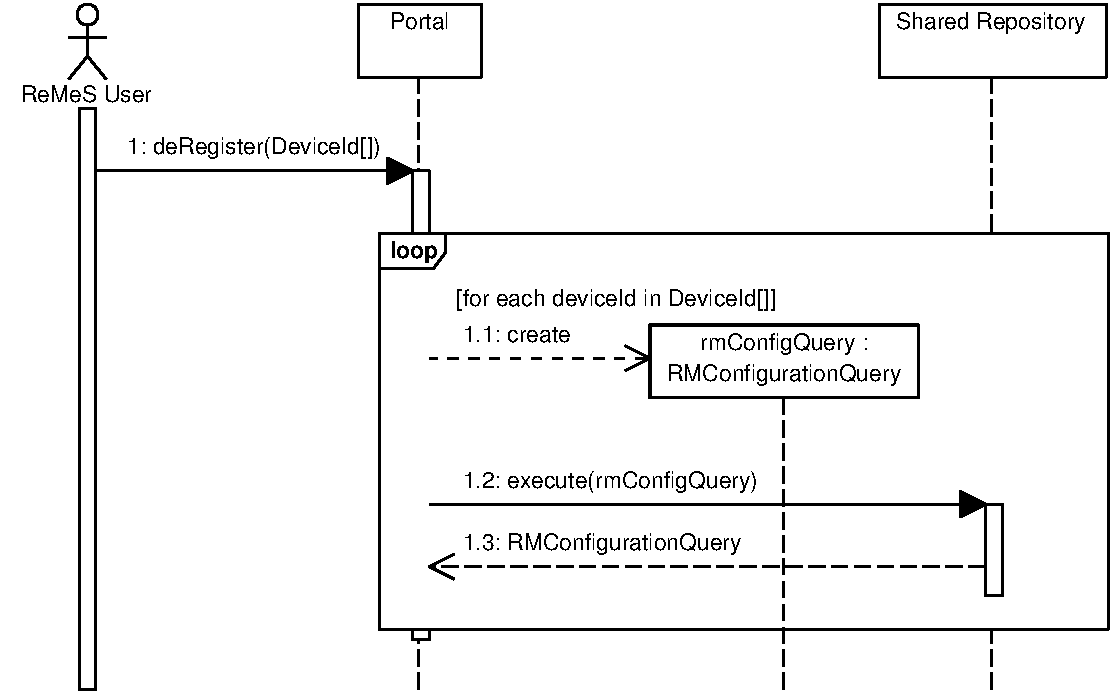
\includegraphics[width=0.7\textwidth]{figs/scenario-5-12.pdf}
		\caption{Sequence diagram for the ``Remote control module de-activation''
		scenario}
		\label{fig:scenario-5-12}
	\end{centering}
\end{figure}

\npar In step 1.1 of figure \ref{fig:scenario-5-12} an RMConfiguarionQuery is
made. This query contains the deviceId to be unregistered, so it is an
update query. This means that the result, RMConfigurationQuery, will in fact be
empty.
